\documentclass[man]{apa}
\usepackage{graphicx,epsfig,amsmath,alltt,setspace,bm}
\title{Studying measurement invariance in factor analysis models
  via stochastic processes}
\twoauthors{Edgar C. Merkle}{Achim Zeileis}
\twoaffiliations{Wichita State University}{Universit\"{a}t Innsbruck}

\abstract{The issue of measurement invariance commonly arises in
  factor-analytic contexts, with methods for assessment
  including 
  likelihood ratio tests, Lagrange multiplier tests, and
  Wald tests.  These tests all require advance definition of the number of
  groups, group 
  membership, and offending model parameters.
In this paper, we construct tests of parameter
invariance based on stochastic processes of casewise
derivatives of the likelihood function.  These tests can be viewed as
generalizations of the Lagrange multiplier test, and they are especially
useful for: (1) isolating specific parameters affected by measurement
invariance violations, and (2) identifying subgroups of individuals
that violated measurement invariance based on a continuous auxiliary
variable.  The tests are presented and illustrated in detail, along
with simulations examining the tests' abilities in controlled conditions.}

\acknowledgements{Correspondence to Edgar C.\
  Merkle, Department of 
  Psychology, Wichita State University, Wichita, KS 67260-0034.
  Email: {\texttt{edgar.merkle@wichita.edu}}.}
\shorttitle{Parameter instability tests}
\rightheader{Parameter instability tests}

\begin{document}
\maketitle

The assumption that parameters are
invariant across observations is a
fundamental tenet of many statistical models.  A specific type of 
parameter invariance, measurement invariance, has implications for the
general design and use of psychometric scales.
This concept is 
particularly important because violations can render the scales
useless.  
That is, if a set of scales violates measurement invariance,
then individuals with the same ``amount'' of a latent variable 
may systematically receive 
different scale scores.
This may lead researchers to conclude subgroup
differences on a wide variety of interesting constructs 
when, in reality, the scales are the sole cause of the 
differences.  Further, it can be inappropriate to incorporate scales
violating measurement invariance into structural equation
models, where relationships between constructs are hypothesized.  Horn
and McArdle \citeyear{HorMca92} concisely summarize the impact of
these issues, stating ``Lack of evidence of measurement 
invariance equivocates conclusions and casts doubt on theory in the
behavioral sciences'' (p.\ 141).  Borsboom \citeyear{Bor06a} also
notes that researchers often fail to assess whether measurement
invariance holds.

In this paper, we consider a new family of tests for assessing
measurement invariance that have important advantages over existing
tests.  We begin by developing a general framework for the tests.
This leads to a discussion of theoretical results relevant to the
proposed tests, as well as a comparison of the proposed tests with
existing tests.  Next,
we study the 
proposed tests' abilities through example and simulation.  Finally,
we discuss some interesting extensions of the tests.
Throughout the manuscript, we use the term {\em{test}} to refer to a
statistical test and the term {\em{scale}} to refer to a psychometric 
test or scale.

\section{Framework}

The tests proposed here are generally relevant to situations where the
$p$-dimensional 
data vector $\bm{x}_i, i=1,\cdots,n$ is specified to arise from a model with
density $f(\bm{x}_i | \bm{\theta}_i)$ and log-likelihood 
$\log L(\bm{\theta}_i | \bm{x}_i)$.  
For the factor-analytic situations
considered in this paper, the $\bm{x}_i$ consist of individuals' scale
scores, and 
$f()$ and $\log L()$ arise from the multivariate normal distribution.
The density is defined as:
\begin{equation}
    \label{eq:mvndensity}
    f(\bm{x}_i | \theta_i) = \frac{1}{(2\pi)^{p/2} |
      \bm{\Sigma}(\bm{\theta}_i) |^{1/2}}\exp(-\frac{1}{2}(\bm{x}_i -
    \bm{\mu}(\bm{\theta}_i))^{\prime} \bm{\Sigma}(\bm{\theta}_i)^{-1} (\bm{x}_i -
    \bm{\mu}(\bm{\theta}_i)),
\end{equation}
where ${\bm{\mu}}({\bm{\theta}}_i)$ is the
model-implied mean vector, and ${\bm{\Sigma}}({\bm{\theta}}_i)$ is the
model-implied covariance matrix.
The casewise log-likelihood is defined as:
\begin{equation}
    \label{eq:caselik}
    \log \text{L}({\bm{x}}_i, {\bm{\theta}}_i) = %\sum_{i=1}^{N} 
\log \mid 
\bm{\Sigma}(\bm{\theta}) \mid + %\sum_{i=1}^{N} 
(\bm{x}_i -
\bm{\mu}(\bm{\theta}))^{\prime} \bm{\Sigma}(\bm{\theta})^{-1} (\bm{x}_i -
\bm{\mu}(\bm{\theta})).
\end{equation}
This equation is often summed over $n$ observations, and it is also
often employed for factor analysis and structural
equation models with missing data (e.g., \citeNP{Wot00}).  We use
the likelihood here to facilitate the proposed tests.

Within the general framework outlined above, model estimation
often proceeds by assuming that $\bm{\theta}_i = \bm{\theta}\
\forall\ i$, then choosing $\hat{\bm{\theta}}$ to satisfy the
criterion:
\begin{equation}
    \label{eq:score}
  \sum_{i=1}^{n} \psi(\bm{x}_i, \hat{\bm{\theta}})] = 0,    
\end{equation}
 where $\psi(\bm{x}_i, \bm{\theta})$ 
is a score function based on the model.  
For example, in factor analysis models estimated via Maximum
Likelihood, the score function is the first derivative of $\log
\text{L}(\bm{x}_i, \bm{\theta})$ with respect to $\bm{\theta}$.
General M-estimation methods may also be handled within this
framework, though we do not discuss them here.

\section{Tests of Measurement Invariance}

Measurement invariance specifically implies that factor analysis model
parameters are invariant across individuals.  It can be framed as the
hypothesis:
\begin{equation}
    \label{eq:h0}
    H_0: {\bm \theta}_i = {\bm \theta}_0,\ i=1,\ldots,n,
\end{equation}
signifying that the parameter vector is the same for all individuals
$i$.  
This general hypothesis is very difficult to test because $n$ is large, and
there are many ways by which the $\bm{\theta}_i$ may stray from one
another.  To circumvent this problem, researchers often measure
individuals on an auxiliary variable $V$ and divide them into groups
based on that variable.  
Assuming a continuous $V$, we might divide 
individuals into two groups based on some threshold $\eta$.
Equation~\eqref{eq:h0} then becomes:
\begin{equation}
    \label{eq:h0.cut}
    H_0: \bm{\theta}_{V < \eta} = \bm{\theta}_{V > \eta},
\end{equation}
where, i.e., $\bm{\theta}_{V < \eta}$ reflects the factor analysis
parameters for all individuals with $V < \eta$.  

Once we have grouped individuals based on $V$,
factor-analytic assessments
of measurement invariance are well developed.
These assessments are often carried out using nested Multiple Groups
Models (e.g., \citeNP{Jor71,Bol89}) coupled with Likelihood Ratio tests,
though 
Lagrange Multiplier and Wald tests may also be constructed for this
purpose.    While these three tests
are asymptotically equivalent \cite{Sat89}, each is detailed
individually below.




% MAY BE USEFUL SOMEWHERE
% Focusing on the latter point, Millsap's \citeyear{Mil05} review of 
% measurement invariance methods cites ``locating the violation of the
% invariance'' as one of the major outstanding problems.  The tests
% resulting from the proposed project directly address this issue,
% leading to an important advance in measurement invariance research.




\subsection{Likelihood Ratio Test}

Measurement invariance is achieved
if sets of factor analysis model parameters are equal across
subgroups of individuals 
(\citeNP{Mer93}; there are many types of measurement invariance based
on different sets of model parameters being held constant, but any of these
can be examined via the proposed tests).  If measurement invariance is
not achieved, 
then the parameters assume different values for different
subgroups.  This leads to statistical tests of measurement
invariance via the comparison of two models: a restricted model where
parameters are equal across subgroups, and a ``full'' model
where parameters are allowed to assume different values for each
subgroup.  Statistically, this comparison is often 
accomplished by a likelihood ratio test (also called a
difference test).  Let the full model parameters be denoted 
${\bm \theta} = ({\bm \theta}_1^{\prime}\ {\bm
  \theta}_2^{\prime})^{\prime}$, where we can obtain the restricted model
by placing a set of equality constraints on ${\bm \theta}_1$ described
by the vector-valued function ${\bm
  h}({\bm \theta}_1) = {\bm 0}$.  A $\chi^2$ statistic testing
measurement invariance may then be calculated via:
\begin{equation}
    \label{eq:chisq}
 \chi^2 = -2(n-1)(\log L({\bm X},
\widehat{{\bm \theta}}_c) - \log L({\bm X},\widehat{{\bm \theta}})),
\end{equation}
where ${\bm{X}}$ is an $n \times p$ data matrix, $\widehat{\bm \theta}_c$
contains Maximum Likelihood parameter estimates satisfying the
constraints ${\bm h}({\bm \theta}_1) = {\bm 0}$, and $\widehat{\bm
  \theta}$ contains Maximum Likelihood parameter estimates from the
full model.  The log-likelihood function in the above equation arises
from the multivariate normal distribution and is defined as:
  The test resulting from
Equation~\eqref{eq:chisq} has 
degrees of freedom equal to the difference in number of free
parameters for the two models, and it rejects the hypothesis of measurement
invariance for large values of $\chi^2$.

While the Likelihood Ratio Test is most popular for testing
measurement invariance, Lagrange Multiplier tests and Wald tests
may also be constructed for the same purpose.The Lagrange Multiplier and Wald 
tests, described below, are also advantageous in that they require
estimation of only one 
model (either the full or restricted model), whereas the Likelihood
Ratio Test requires estimation of both models.

\subsection{Lagrange Multiplier Test}
The Lagrange Multiplier test (e.g., \citeNP{Sil59,ChouBent90})
focuses on a restricted model and tests whether the equality
constraints described by ${\bm h}({\bm \theta}_1) = {\bm 0}$ should be
freed.
Estimating the restricted model, we define a vector of Lagrange
multipliers $\widehat{\bm \kappa}$ that satisfy:
\begin{equation}
    \label{eq:lagrange}
    \frac{\partial \log L}{\partial {\bm \theta}} \bigg |_{\widehat{\theta}_c} +
    \frac{\partial {\bm h}}{\partial {\bm \theta}}
    \bigg |_{\widehat{\theta}_c}^{\prime} \widehat{{\bm \kappa}} = {\bm 0}.
\end{equation}
The test itself is then based on the asymptotic distribution of 
$\widehat{{\bm \kappa}}$: if $\widehat{{\bm \kappa}}$ is sufficiently close
to ${\bm 0}$, then the constraints are deemed to hold in the
population.  The resulting test statistic, which is a function of
$\widehat{\bm \kappa}$, follows a $\chi^2$ distribution for large
samples.

\subsection{Wald Test}
In contrast to the Lagrange Multiplier test, the
Wald test (e.g., \citeNP{Wald43})
focuses on the full model and tests the plausibility of the
constraints ${\bm h}({\bm \theta}_1) = {\bm 0}$.
The test is based on the estimates ${\bm h}(\widehat{{\bm \theta}}_1)$
from the full model; if
these are sufficiently close to zero, then the constraints are deemed
to hold in the population.  The resulting test statistic, which is a
function of ${\bm h}(\widehat{{\bm \theta}}_1)$, is also
$\chi^2$-distributed in large 
samples.
Chou and Bentler \citeyear{ChouBent90} compared the 
Wald and Lagrange tests with finite sample sizes via
simulation, and they generally found similar
performance.  They noted, 
however, that the Lagrange test has a tendency toward Type I errors in
some contexts.  They therefore urged caution in the Lagrange test's
use, as it may lead one to discard more constraints than is necessary,
leading to overly-complex models.

\subsection{Extensions to Proposed Tests}
For continuous $V$, the three tests described above require the
threshold $\eta$ to be known.
  This is a
major limitation in psychometrics, where $\eta$ is often unknown or
undefined.
For example, if $V$ represents yearly income, there are many possible
values of 
$\eta$ that could be used to divide individuals into poorer and richer
groups.  The ultimate $\eta$ that we
choose could potentially impact our
conclusions about whether or not a scale is measurement invariant, 
in the same way that dichotomization of continuous variables impacts
general statistical analyses \cite{MacZha02}.

Instead of choosing a specific $\eta$, we may elect to test
individuals across all possible values of $\eta$.  For example, we
could conduct a Likelihood Ratio Test for every possible
dichotomization of $V$, yielding a test statistic for each
dichotomization.  The distribution of the maximum of these test
statistics is derived in Andrews \citeyear{And93}, providing a test of
measurement invariance over all values of $\eta$.  
This is a special case of the family of tests proposed here.  The
tests are designed for situations where
$\eta$ is unknown or where a dichotomization of $V$ is insufficient to
detect measurement invariance violations, and they can be applied both
to individual model parameters and sets of model parameters.

We now describe some general ideas for capturing measurement
invariance violations with respect to a continuous auxiliary variable
$V$.



\section{Stochastic Processes for Measurement Invariance}
The proposed tests of measurement invariance implicitly rely on an
estimated factor analysis model (one that restricts parameters to be
invariant across subgroups).  For the purposes of this paper, we
assume that the model is estimated via Maximum Likelihood.  
The factor analysis log-likelihood may be obtained by summing 
Equation~\eqref{eq:caselik} across individuals.  
Maximization of the likelihood then involves iterative 
algorithms that seek values $\widehat{{\bm{\theta}}}$ to satisfy
Equation~\eqref{eq:score}, where 
$\psi(\bm{x}_i, \theta_j) = \frac{\partial}{\partial \bm{\theta}} \log
\text{L}({\bm{x}}_i, 
{\bm{\theta}}) \big |_{\bm{\theta} = \widehat{\bm{\theta}}}$.
% insert derivatives of casewise evaluated at theta-hat = 0
Such derivatives are taken across individuals, but, using individual
terms of the log-likelihood (i.e., Equation~\eqref{eq:caselik}),
we can also 
evaluate the derivatives with respect to each individual.
If a unique value of $\widehat{{\bm{\theta}}}$ maximized
each individual likelihood, then we would have:
% Equation: \psi(y_i, \theta) = d/d theta casewise_i = 0 \forall i.
\begin{equation}
    \label{eq:casederiv}
    \psi({\bm{x}}_i, \bm{\theta}) = \frac{\partial}{\partial \bm{\theta}} \log
\text{L}({\bm{x}}_i, 
{\bm{\theta}}) \bigg |_{\bm{\theta} = \widehat{\bm{\theta}}} = \bm{0}\ \ \ \forall\ i.
\end{equation}
In practice, no value of $\widehat{{\bm{\theta}}}$ will maximize all
individuals' likelihoods, but, if measurement invariance is satisfied, 
we can expect the $\psi(\cdot, \cdot)$ to fluctuate around zero.  This
is the idea underlying the tests described here.

\subsection{Theory}
Theoretical work in statistics (e.g.,
\citeNP{BroDur75,HjoKon02,Nyb89}) has shown 
that functions of the 
$\psi(\cdot, \cdot)$ follow specific stochastic processes, allowing
us to use them to generally test measurement
invariance.  
We rely on the null hypothesis specified in Equation~\eqref{eq:h0},
which focuses on individuals instead of groups of individuals.
We now review some of the main results
for testing this $H_0$; more
detailed accounts include Hjort and Koning \citeyear{HjoKon02} and
Zeileis and Hornik \citeyear{ZeiHor07}.

% New subsection starts here?

For application to measurement invariance, the most important
theoretical result involves the fact that, under $H_0$, functions of
the $\psi(\cdot, \cdot)$ result in specific stochastic
processes.  One such function
is the {\em{cumulative score process}}, given as:
\begin{equation}
    \label{eq:cumscore}
    W_n(t,\theta_j) = \frac{1}{\sqrt{n}} \sum_{i=1}^{\lfloor nt
      \rfloor} \psi ({\bm{x}}_i, \theta_j),
\end{equation}
where $t$ is a continuous variable in $(1/n,1)$ and $\lfloor nt
\rfloor$ is the floor operator, defined as the integer part of
$nt$.
As the equation shows, the cumulative score process adds subsets of
casewise first derivatives across individuals who have been ordered
based on an auxiliary variable.  Starting at $t=1/n$, only the
first individual's derivative enters into the summation.  Once
$t=2/n$, the first two individuals' derivatives enter into the
summation.  This procedure continues until we reach $t=n$, at which
point all individuals' first derivatives have entered into the
summation.  There are $n$ cumulative sums obtained by sequentially
inserting individuals' derivatives into the equation, and these are
calculated 
for each of the $p$ model parameters.  This results
in $n\times p$
empirical cumulative scores.

Elements of the summation in Equation~\eqref{eq:cumscore}
can be positive or 
negative, so that the cumulative scores do not necessarily increase
with $t$.  In fact, if measurement invariance (i.e., $H_0$) holds,
then the cumulative scores should 
follow a stochastic process that fluctuates around zero.  
Zeileis and Hornik \citeyear{ZeiHor07} showed specifically that, under
$H_0$:
\begin{equation}
    \label{eq:browbridge}
{\bm{B}}(\cdot, \widehat{{\bm{\theta}}}) = {\bm{I}}(\widehat{{\bm{\theta}}})^{-1/2}{\bm{W}}_n(\cdot,\widehat{{\bm{\theta}}})
\overset{d}{\rightarrow} {\bm W}^{0}(\cdot), % put d over rightarrow
\end{equation}
where ${\bm{I}}(\widehat{{\bm{\theta}}})$ is the observed information
matrix (e.g., of the factor analysis model), ${\bm{W}}_n(\cdot,\widehat{{\bm{\theta}}})$ reflects the $p$-dimensional
cumulative sums (one for each parameter), ${\bm W}^{0}(\cdot)$ is a
$p$-dimensional Brownian bridge, and 
$\overset{d}{\rightarrow}$ reflects convergence in distribution.
In words, there are $p$ cumulative score processes, one for each
model parameter.  This collection of processes follows a
multidimensional Brownian bridge as derivatives accumulate in the 
summation from individual 1 to individual $n$.
Multiplication by ${\bm{I}}(\widehat{{\bm{\theta}}})^{-1/2}$ 
``decorrelates'' the $p$
cumulative score processes, such that each univariate process (i.e., each
process for a single model parameter) is unrelated to all other
processes (and is asymptotically independent of the other processes).

The cumulative scores resulting from Equation~\eqref{eq:browbridge}
can be arranged in an $n \times p$ matrix called an {\em{empirical
    cumulative score process}}, which we will denote as
${\bm{B}}^{\ast}(\widehat{\bm{\theta}})$.
Each column of this matrix follows a univariate Brownian bridge and is
based on a single factor analysis parameter. 
To carry out a test of $H_0$, we need functions that collapse across
rows (individuals) and/or columns (parameters) of the matrix.  
These
functions then lead to scalar test statistics and p-values.
The specific choice of function depends on the goals of the analyst:
the row-collapsing functions are useful for isolating subsets of
parameters that violate measurement invariance, and the
column-collapsing functions are useful for isolating subgroups of
individuals who violate measurement invariance across all parameters.
Some functions result in test
statistics whose critical values can be derived analytically, while
others require critical values to be derived via the
simulation of a Brownian bridge.

For example, if we wish to test a specific parameter for
measurement invariance, ``row-collapsing''
functions include the absolute maximum or mean of the corresponding 
column in ${\bm{B}}^{\ast}(\widehat{\bm{\theta}})$
\cite{ZeiHor07}. % (see ZH07 p 7)
Conversely, if we wish to generally test 
measurement invariance across sets of model parameters,
``column-collapsing'' functions 
include the maximum norm or the squared Euclidean norm of the
corresponding row in ${\bm{B}}^{\ast}(\widehat{\bm{\theta}})$
\cite{HjoKon02}.

% A general, two-step strategy for testing measurement
% invariance involves first collapsing over columns for each individual,
% yielding a single statistic for each individual. 
% These $n$ statistics (ordered according to an auxiliary variable)
% can then be graphed to visually define groups that violate measurement
% invariance.  Functions of these $n$ statistics can also yield scalar
% test statistics.

As a concrete example of these ideas, consider the situation
where we carry out a Likelihood Ratio test for all possible values of
$\eta$, then take the maximum of these test statistics.  A related
idea here involves taking the maximum of the empirical cumulative
score process:
\begin{equation}
    \label{eq:doubmax}
    DM = \max_{i=1,\ldots,n} \max_{j=1,\ldots,p} |
    B^{\ast}_{ij}(\widehat{\bm{\theta}}) |,
\end{equation}
where $B^{\ast}_{ij}(\widehat{\bm{\theta}})$ represents the
entry in row $i$ and column $j$ of
${\bm{B}}^{\ast}(\widehat{\bm{\theta}})$.
This is a 
{\em{double-max}} statistic that allows for simultaneous isolation of 
$\eta$ along with model parameters that change over $\eta$.
This statistic is
especially useful for visualization, as the fluctuation process for
each individual parameter can be displayed along with the appropriate
critical value.  An example of this visualization appears in the
Example section.

As a second example of ``collapsing'' functions,
we could first collapse over columns for each individual $i$ via the
Euclidean norm:
\begin{equation}
    \label{eq:meanl2}
    \nu_i = \lVert {\bm B}^{\ast}_{i\cdot}(\widehat{\bm \theta}) \rVert,
\end{equation}
where the $i\cdot$ subscript signifies row $i$ of the empirical
fluctuation process matrix.  A univariate test statistic may then be
obtained by taking the mean of the $\nu_i$.  This is a
Cram\'{e}r-von Mises statistic described by, e.g., Nyblom
\citeyear{Nyb89} and Hansen \citeyear{Han92} in the contexts of
longitudinal models and linear regression.  In general contexts,
this test is recommended
when there are more than two groups exhibiting parameter instability 
and when multiple parameters change across groups \cite{ZeiSha10}.  
We demonstrate these recommendations' implications for
measurement invariance later in the paper.

% We still obtain a unidimensional process; the norm is applied
% to each row vector.
There exist other functions of first derivatives and of the
empirical fluctuation process that
result in other test statistics; these are described by, e.g.,
Zeileis, Shah, and Patnaik \citeyear{ZeiSha10}.  
In the analyses described later, we focus on the abilities
of the Cram\'{e}r-von Mises test and of the double-max test.  However,
the many 
row- and column-collapsing functions offer a large family of tests
that can be applied to the study of measurement invariance.

\subsection{Critical Values \& $p$-values.}
To obtain $p$-values associated with $H_0$, we can rely on analytic
work concerning functions of Gaussian processes.
As an example of this, we focus on use of the 
double-max function (Equation~\eqref{eq:doubmax}) as a test statistic.
There exist 
analytic results for Brownian bridges that allow us to calculate
% fix double-max notation on following line:
$P(DM > \beta | H_0)$, where $\beta$ is a specific value
that the test statistic may achieve.  

Focusing on a univariate
Brownian bridge under $H_0$, it can be shown that (e.g., \citeNP{ShoWel86}):
 % see Beghin & Orsingher Eq (4.12).  They cite Shorack &
            % Wellner 1986 book
\begin{eqnarray}
    P(DM_j < \beta | H_0) &
    = & \sum_{h=-\infty}^{\infty} (-1)^h \exp(-2h^2\beta^2) \\
   & = & 1 + 2 \sum_{h=1}^{\infty} (-1)^h \exp(-2h^2\beta^2).
\end{eqnarray}
The associated $p$-value is therefore given by:
\begin{equation}
    \label{eq:absmax_p}
        p = P(DM_j > \beta | H_0)
    = 1 - (1 + 2 \sum_{h=1}^{\infty} (-1)^h \exp(-2h^2\beta^2)).
\end{equation}
The terms in the summation quickly go to zero as $h$ goes to infinity,
so, in practice, we only need to compute the first 100 terms (say).
For multidimensional Brownian bridges whose dimensions have been
``decorrelated'', $p$-values can
be obtained similarly with a Bonferroni correction.

For the Cram\'{e}r-von Mises test statistic, analytic expressions for
$p$-values are more cumbersome.  Nyblom \citeyear{Nyb89} and Hansen
\citeyear{Han92} provide small tables of critical values, and other
critical values are easily approximated via simulation of Brownian
bridges.

\subsection{Locating the Invariance.}
If a test described above implies a measurement invariance violation,
then the researcher may want to: (1) estimate $\eta$, so that she may
define subgroups of individuals impacted by measurement invariance;
or (2) isolate model
parameters affected by the invariance.  
In the context of a Cram\'{e}r-von Mises test, we can accomplish the
first task by graphing the $\nu_i$ (Equation~\eqref{eq:meanl2})
and noting the location of the peaks and valleys.  We can accomplish
the second task by taking the norm in Equation~\eqref{eq:meanl2}
across specific columns of $B^{\ast}(\widehat{\bm \theta})$.

In the context of a double-max test, we can accomplish the first task
by defining $\eta$ to be the value
of $V$ at which the absolute
maximum cumulative score is achieved.  This value maximizes the
segmented likelihood, defined as:
\begin{equation}
    \label{eq:seglik}
    \sum_{i; V_i \leq \eta} L(\bm{x}_i, \bm{\theta}_{V \leq \eta}) + 
     \sum_{i; V_i > \eta} L(\bm{x}_i, \bm{\theta}_{V > \eta}).
\end{equation}
where $\bm{\theta}_{V \leq \eta}$ and $\bm{\theta}_{V > \eta}$ are ML estimates
for individuals with 
$V_i \leq \eta$ and with $V_i > \eta$, respectively.
  For multiple thresholds, we
could heuristically define groups based on the number of peaks and
valleys in the graph, or we could maximize a segmented likelihood
similar to that in Equation~\eqref{eq:seglik}.
We can accomplish the second task (isolating model parameters) by
conducting posthoc 
tests on specific model parameters.  
%Some of these ideas are illustrated in
%the example below.

\begin{figure}
\caption{Path diagram representing the base factor analysis model used for
  the Example and Simulations.  To induce measurement invariance
  violations, a seventh observed variable (student age) determines the
values of the verbal factor loadings ($\lambda_{11}$, $\lambda_{21}$,
$\lambda_{31}$).}
\label{fig:famod}
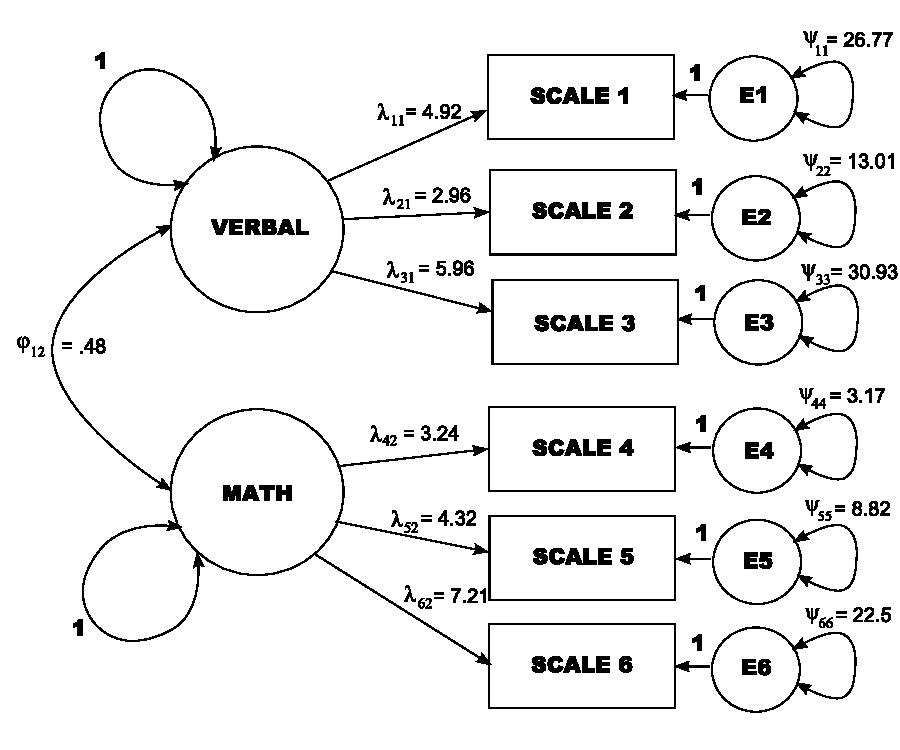
\includegraphics[height=5in]{famod.pdf}
%\input{figs/path}
\end{figure}

\section{Example with Artificial Data}

As an example of the ideas discussed above, consider a
hypothetical battery of six scales administered to students aged 14 to 17
years.  Three of the scales are intended to measure verbal ability, and
three of the scales are intended to measure mathematical ability.  We
may observe a maturation effect in the resulting data, whereby the scales
measure older students better than younger students (i.e., the scales
are too difficult for younger students).  The researcher's goal is to
study whether the scales are measurement invariant with
respect to age, which is taken to be the auxiliary variable $V$.

\subsection{Method}

To formally represent these ideas, we specify that the data arise from
a factor analysis model with two factors.  The base model, displayed in
Figure~\ref{fig:famod}, specifies that measurement invariance holds,
with three scales arising from the verbal factor and three 
scales arising from the mathematical second factor.
For measurement invariance violations, we specify that $V$
(student age) impacts the values of 
verbal factor loadings in the model: 
if students are 16 or 17 years of age, then the factor
loadings corresponding to the first 
factor ($\lambda_{11}, \lambda_{21}, \lambda_{31}$) reflect those in
Figure~\ref{fig:famod}.  If students are 14 or 15 years of age,
however, then the factor loadings corresponding to the first factor
are three standard errors lower than those in Figure~\ref{fig:famod}
(the standard errors were obtained by fitting
  the model to a sample of size 200, where the sample consisted of all
  ``older'' subjects).
This violation states that the verbal ability scales
lack measurement invariance with respect to age.  For simplicity, we
assume that the mathematical scales are invariant.



A sample of size 200 was generated from the model described above, and
a test was conducted to examine measurement invariance of the three
verbal scales.  To carry out
the test, a confirmatory factor analysis model (with the paths
displayed in Figure~\ref{fig:famod}) was fit to the
data.  Casewise derivatives and 
the observed information matrix were then obtained, and they were used
to calculate the cumulative score process via
Equations~\eqref{eq:cumscore} and~\eqref{eq:browbridge}.  Finally, we
obtained a 
double-max statistic via Equation~\eqref{eq:doubmax} and associated
$p$-value via Equation~\eqref{eq:absmax_p}.  Note that, because we
were examining only the three verbal factor loading parameters, the
specific null hypothesis being tested is:
\begin{equation}
    \label{eq:exh0}
H_0:\ (\lambda_{i,11}\ \lambda_{i,21}\ \lambda_{i,31}) =
(\lambda_{11}\ \lambda_{21}\ \lambda_{31}),\ i=1,\ldots,n,
\end{equation}
where $(\lambda_{i,11}\ \lambda_{i,21}\ \lambda_{i,31})$ represent the
verbal factor loading parameters for student $i$.

\subsection{Results}
In the results section, we first describe overall results and then 
describe estimation of $\eta$ and 
isolation of model parameters violating
measurement invariance.

\subsubsection{Overall Results}
Results related to the cumulative score process are displayed in
Figure~\ref{fig:cusumex}.  In this figure, the processes
are displayed individually 
for each factor loading, with student number (ordered by age and
rescaled to (0,1)) on the x-axis and
absolute values of the cumulative scores on the y-axis.  The dashed horizontal
lines represent the critical value for rejecting $H_0$ at $\alpha=.05$
based on the double-max statistic; if any of the three processes
crosses the horizontal line, then we reject $H_0$.  It is seen that
the processes for both the second and third factor loadings
($\lambda_{21}$ and $\lambda_{31}$) cross the dashed line, indeed
implying rejection of $H_0$.  The maximum across all three processes,
corresponding to the double-max test statistic, is 1.72.  This maximum
occurs in the third graph and is represented as a solid circle, 
achieving a $p$-value of .016.  



\subsubsection{Estimation of $\eta$ and Parameter Isolation}
The results of the test imply that the 
verbal scales lack measurement invariance, and the age at which the
maximum is achieved provides the estimate $\hat{\eta}$.
The student corresponding to the maximum
absolute cumulative sum (the solid circle in the third graph) is 15.8
years of age, implying one subgroup of 
students below 15.8 years and one above 15.8 years.  This agrees well
with the true $\eta$ of 16.0 years.

The results of the test also yield information about specific
parameters violating measurement invariance.  We simultaneously tested
three factor loading parameters for measurement invariance.  Given
rejection of the hypothesis of measurement invariance, we can 
do posthoc 
tests to study specific parameters violating measurement invariance.
This involves individual examination of each cumulative score process
(i.e., of each of the three graphs in Figure~\ref{fig:cusumex}),
along with a procedure that controls for Type I error.  Taking a
Bonferroni approach, we can examine whether each process's maximum
surpasses the critical value associated with an $\alpha$ of
$.05/3=.017$.  This amounts to the same critical value as that used in
the overall test, 
meaning that we simply examine the individual processes that cross
the horizontal dashed lines in Figure~\ref{fig:cusumex}.  The figure
shows that the second and third parameters (i.e., $\lambda_{21}$ and
$\lambda_{31}$) cross the dashed line, so we would conclude a measurement
invariance violation with respect to age in the second and third
verbal tests.  The fact that the cumulative score process for
$\lambda_{11}$ did not achieve the critical value represents a Type II
error, which implicitly brings into question the posthoc tests' power.  We
generally address the issue of power in the simulations below.

\begin{figure}
\caption{Cumulative score processes for the verbal factor loadings,
  based on the example involving measurement invariance with respect
  to student age.  The dashed lines represent critical values for the
  test of measurement invariance at $\alpha=.05$.}
\label{fig:cusumex}
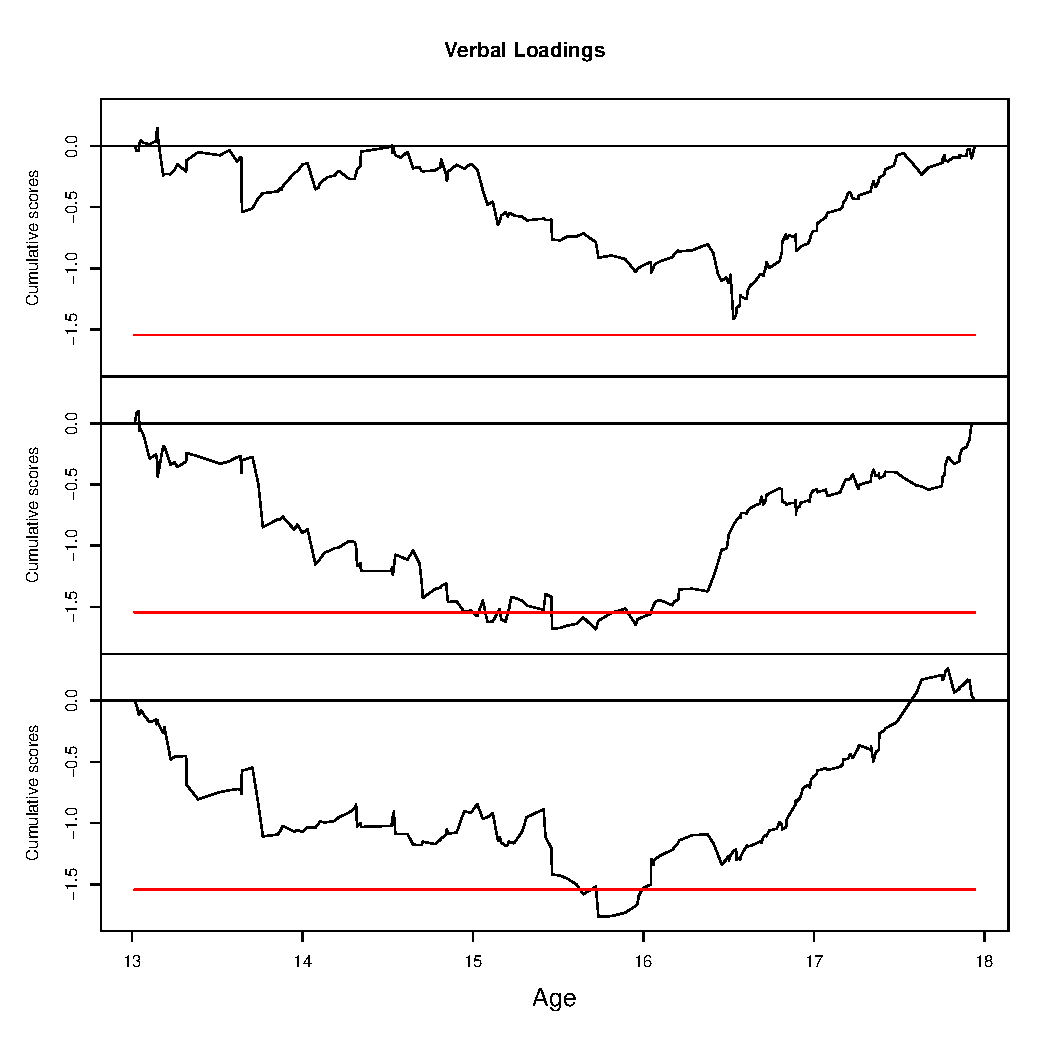
\includegraphics[height=5in]{example.pdf}
\end{figure}

\section{Simulation}
% Simulations demonstrating power of test(s) at various
% sample sizes, types of invariance violations, ?
In this section, we conduct a simulation designed to
examine the tests' power and Type I error rates in the context
described previously (testing three factor loadings for measurement
invariance).  We 
examine the power and error rates of three tests: the double-max test, the
Cram\'{e}r-von Mises test, and the traditional likelihood
ratio (difference) test involving nested 
multiple-group models.  The likelihood ratio test has an advantage over the
other two tests here, in that it requires advance definition of
$\eta$.  This test is useful for comparative purposes,
however, as it helps indicate the extent to which the other tests
``lose'' power due to $\eta$ being unknown.

\subsection{Method}
Simulated data were generated in a similar way to that of 
the Example section.
The data included verbal scales that violated measurement invariance
with respect to students' ages, with students 14--15 years of age
having smaller factor loadings than students 16--17 years of age.  
Simulation data were generated from the same general factor analysis
model (see Figure~\ref{fig:famod}), but sample size and magnitude
of measurement 
invariance violation was manipulated to examine power:
we examined power to detect 
invariance violations across three sample sizes ($n=100,
200, 500$) and three magnitudes of violations (factor loadings
for the younger students being 0, 1, 2, or 3 standard
errors\footnote{The standard errors used here were
  obtained by fitting
  the model to a sample of size 100, where the sample consisted of all
  ``older'' subjects.} below 
those for the older students).  The 0-standard error condition was
used to study Type I error rate.

For each sample size $\times$
magnitude combination, 500 datasets were generated and tested for
measurement invariance.  For the 0-standard error condition, we
generated 5,000 datasets because small proportions are more
 difficult to estimate precisely.  In each dataset, half the
students were 14--15 
years of age and half were 16--17 years of age.  As stated previously,
group
designations ($\eta$) were assumed to be
known for the likelihood ratio test.

\subsection{Results}
% MODIFY RESULTS TO DISCUSS ALL THREE TESTS
% ALSO NEED 0-SE CONDITION
For each test statistic, power and Type I error rates for the twelve
sample size $\times$ magnitude combinations are displayed in
Table~\ref{tab:sim1}.  The 0-SE column lists Type I error rates; this
is the situation where the tests reject the hypothesis of measurement
invariance at $\alpha=.05$ when none exist.  This column 
shows that the Cram\'{e}r-von Mises test has accurate Type I error
rates at all sample sizes examined.
The double-max test, on the other hand, is conservative at
all sample sizes examined.  Finally, the likelihood ratio test is
slightly liberal at smaller sample sizes, with Type I error rates of
.07 and .06 at $n=100$ and $200$, respectively.  Type I error for the
likelihood ratio test at $n=500$ is accurate, however.

Focusing on power, the table includes many interesting results.
First, the likelihood ratio test has superior power over the stochastic
process-based tests at all sample sizes and invariance violations.
This is likely due to the fact that the likelihood ratio test had
extra information ($\eta$), whereas the other tests
were testing measurement invariance over all values
of $\eta$.  While power was lower for the tests developed in this
paper, it was not terribly low.  At $n=200$ and above, all tests were
on the same side of the traditional power cutoff of 0.8.  The tests
were able to detect large measurement invariance violations (of three
and sometimes two standard errors) at the larger sample sizes, and
they were generally unable to detect the one-standard-error violation
at any of the sample sizes studied.

Comparing only the two proposed test statistics, we see that the
Cram\'{e}r-von Mises test has better power in all conditions.  This is
similar to the general recommendation described by Zeileis et al.\
\citeyear{ZeiSha10}, stating that the Cram\'{e}r-von Mises test
is generally superior when multiple parameters change simultaneously.
Because the three verbal factor loadings all changed
across the two subgroups in the simulation, the Cram\'{e}r-von Mises
test excels.

In summary, we found that the proposed tests have less power than a
likelihood ratio test with known subgroups.  However, the power levels
remain adequate after considering the fact that the proposed tests are
testing measurement invariance across all possible subgroups.  For the
two-factor model examined here, all tests had trouble detecting small
measurement invariance violations at small sample size.  Larger
violations were more easily detected at larger sample sizes, with the
Cram\'{e}r-von Mises test having better power due to multiple
parameters being involved in the invariance violation.

% 0-SE column is fixed for n=100 (using 5000 reps instead of 500)
\begin{table*}
\caption{Simulated power and Type I error rates for three test statistics
  across three sample sizes and four magnitudes of measurement
  invariance violations. Abbreviations: CvM = Cram\'{e}r-von Mises
  test; DM = Double-max test; $\chi^2$ = Chi-square likelihood ratio
  test.}
\label{tab:sim1}
\begin{tabular}{llcccc} \thickline
 & & \multicolumn{4}{c}{Violation Magnitude (SEs)} \\
$n$ & Test Stat & 0 & 1 & 2 & 3 \\\hline
100 & CvM       & 0.05 & 0.10 & 0.33 & 0.63 \\ 
    & DM        & 0.03 & 0.06 & 0.19 & 0.41 \\ 
    & $\chi^2$  & 0.07 & 0.16 & 0.49 & 0.83 \\ \hline
200 & CvM       & 0.05 & 0.19 & 0.64 & 0.96 \\ 
    & DM        & 0.03 & 0.12 & 0.44 & 0.88 \\ 
    & $\chi^2$  & 0.06 & 0.27 & 0.76 & 0.99 \\ \hline
500 & CvM       & 0.05 & 0.44 & 0.98 & 1.00 \\ 
    & DM        & 0.04 & 0.35 & 0.94 & 1.00 \\ 
    & $\chi^2$  & 0.05 & 0.58 & 1.00 & 1.00 \\\thickline
\end{tabular}
\end{table*}







% Need to re-do simulation to monitor specific parameters in the
% posthoc test.

% Cramer-von Mises now in Sim 1.  May skip Sim 2 for the time being.
%\section{Simulation 2: Improving Power}
%Simulation 2 examines whether we can improve power using a Cramer-von
%Mises statistic (summing instead of taking maximum).

% Table 2 of Nyblom89 contains critical values that may prove useful.
% Hansen 1992 p. 524 has table of critical values that matches 
%  Nyblom89 within reason.
% See Zeileis05 p. 450-451



% Use model that is similar to the example.

\section{Discussion}
In this paper, we have presented a new family of statistical tests for
the study of measurement invariance in psychometrics.  The tests,
based on stochastic processes, have reasonable power, can isolate
groups of individuals violating measurement invariance based on a
continuous, auxiliary variable, and can
isolate specific model parameters affected by the violation.  In this
section, we consider the tests' use in practice and their 
extension to more complex scenarios.

\subsection{Use in Practice}
% Simultaneous test of Meredith's various types of invariance
The proposed tests give researchers a new set of tools for studying 
measurement invariance.  For example, they give researchers the
opportunity to simultaneously test for many types of measurement
invariance (see, e.g., \citeNP{Mer93}).  The traditional
steps have involved hypothesizing a specific type of invariance and
then testing for it via a Likelihood Ratio Test, but the tests
proposed here do not require one to hypothesize a specific type of
invariance a priori.  Instead, one could define a type of measurement
invariance after seeing the proposed tests' results.

% Researchers interpreting subgroups violating MI
In addition to simultaneously testing different types of measurement
invariance, the proposed tests allow researchers to easily interpret
the nature of the invariance violation.  This is made possible through
the tests' abilities to estimate $\eta$, the threshold dividing
individuals into subgroups that violate
measurement invariance.  While a single $\eta$ was estimate in this
paper, it is also possible to define 
formal rules for estimating multiple $\eta$ parameters.  We plan to
explore these ideas in the future.

% \subsection{Further Issues}
% Further issues associated with the proposed tests include: (1)
% alternative methods for estimating $\eta$;
% and (2) dealing
% with categorical $V$.  We address each in turn below. 

% % More than two groups violating MI
% \subsubsection{Estimation of $\eta$}
% Given rejection of the hypothesis of measurement invariance, the most
% straightforward way to formally estimate $\eta$ is through
% the location of the maximum of the cumulative score process.  Assuming
% a single threshold, the maximum should be achieved close to the true
% $\eta$.  Referring to the Example (see
% Figure~\ref{fig:cusumex}), we defined $\eta$ as the 
% age corresponding to the solid dot in the third panel.

% To study this method in more detail, we used
% results of our simulation to examine the age at which the maximum of
% the cumulative score process occurs.
% If the test accurately recovers the violating subgroups,
% then the maximum should be close to 16 years
% of age.\footnote{The data generated for these
%   simulations 
%   contained ages measured in days, as opposed to years.  Thus,
%   the tests could split students at continuous values like 15.6 or
%   16.3 years of age.}
%   For each simulation condition, Table~\ref{tab:age1}
%   displays confidence intervals for the location of the maximum
%   absolute cumulative score.  These confidence intervals were
%   calculated across generated 
%   datasets, with each dataset contributing one maximum absolute cumulative
%   score
%   (regardless of whether the hypothesis of
%   measurement invariance was rejected).
% It is observed that these confidence intervals slightly underestimate
% the true age dividing the subgroups, with the degree of bias
% decreasing as sample size increases.  The interval widths
% are impacted by both the magnitude of the invariance and the sample
% size.  In future work, we plan to study alternative ways of
% identifying subgroups.

% \begin{table*}
% \caption{Confidence intervals for the location of the maximum absolute
%   cumulative score across the conditions from the simulation.}
% \label{tab:age1}
%   \begin{tabular}{lccc} \thickline
%   & \multicolumn{3}{c}{Violation Magnitude} \\
%   $n$ & 1SE & 2SE & 3SE \\\hline
%   100 & (15.61; 15.73) & (15.55; 15.65) & (15.50; 15.59) \\
%   200 & (15.67; 15.77) & (15.64; 15.72) & (15.67; 15.73) \\
%   500 & (15.71; 15.81) & (15.77; 15.83) & (15.80; 15.83) \\\thickline
%   \end{tabular}
% \end{table*}

% Differing proportions of people in each group
%\subsubsection{Subgroup Proportions}
%The power of the proposed tests is impacted by the proportion of
%individuals within each subgroup.  

% Ties on auxiliary variable (mention use in categorical contexts)
\subsection{Categorical Auxiliary Variable}
% There remain unaddressed theoretical issues specific to the 
% tests' application to measurement invariance.  These
% issues generally stem from the types of auxiliary variables on which
% researchers may study measurement invariance.  In
% the example described earlier, researchers wanted to know whether a
% scale was measurement invariant with respect to student age.
% Students could then be ordered based on age, and a test could be 
% constructed via Equation~\eqref{eq:cumscore}.  However, an issue arises if there
% are ties on age; that is, if two students' ages are exactly
% the same.  The proposed tests assume complete ordering of the
% students, but these two students cannot be ordered.  In this case, we
% may randomly order the two students, but there is an
% arbitrariness associated with this strategy.  Alternatively, to obtain
% tests that liberally reject the hypothesis of measurement invariance,
% we may choose the ordering that results in the largest test
% statistic.  If there are many tied students, then there are many
% possible orderings that must be examined.  However, examination of all
% possible orderings remains computationally feasible because the
% casewise first derivatives need to be calculated only once; the
% derivatives simply need to be reordered for each ordering of tied
% students.

One issue that was largely unaddressed in this paper involved the use
of categorical $V$ to study measurement invariance.  In this case,
groups are 
already specified in advance, and so traditional methods (i.e.,
Likelihood Ratio tests) may suffice.
However, we could use the framework developed here to obtain an
alternative $\chi^2$ statistic testing measurement invariance.
Assume the observations are divided into $K$ categories $I_1, I_2,
\ldots, I_K$.
First, we can sum scores within each category of the
demographic variable via:
\begin{equation}
    \label{eq:catsum}
    \Delta W_n(I_k) = \frac{1}{n_k\sqrt{n}} \sum_{i \in I_k}
    {\bm{I}}(\widehat{\bm{\theta}})^{-1/2} {\bm{\psi}}({\bm{y}}_i, \widehat{{\bm
      \theta}}),
\end{equation}
where $n_k$ is the sample size in category $k$ and $n$ is the overall
sample size.  This results in a $K \times p$ matrix, with one entry for
each category-by-model parameter combination.  We can test
a specific model parameter for invariance by focusing on the associated
column of the $K \times p$ matrix, summing over the squared entries in
the column to obtain a $\chi^2$ statistic with
$(K-1)$ degrees of freedom \cite{HjoKon02}.
Alternatively, to simultaneously test multiple parameters, we can sum
the $\chi^2$ statistics and degrees of freedom for the individual
parameters.

\subsection{Extensions}
The proposed family of tests can be extended in various ways.  First,
it is possible to construct an algorithm that recursively defines
groups of individuals violating measurement invariance with respect to
multiple auxiliary variables.  Such an algorithm is related to 
classification and regression trees \cite{BreFri84,MerSha10,StrMal09},
and related algorithms have been developed for generalized linear
models \cite{ZeiHot08} and Rasch models \cite{KopZei10}.

% Recursive method
% \subsubsection{Recursive Multiple-Groups Models}
% The proposed tests have the ability to automatically define groups of
% individuals violating measurement invariance with respect to a single
% auxiliary (often demographic) variable.  If a researcher has multiple
% auxiliary variables that he/she wishes to assess for measurement
% invariance, then the proposed tests can be inserted into a recursive
% algorithm 
% that isolates groups of individuals violating measurement
% invariance.   and
% C4.5 \cite{Qui93}.  The algorithm would proceed via the following
% steps: 
% \begin{enumerate}
%   \item Fit a confirmatory factor analysis model to the data, with all
%   parameters constrained to be equal across observations.
%   \item Conduct a measurement invariance test with respect to each
%     auxiliary variable (auxiliary variables are determined in
%     advance by the researcher).
%   \item If violations of measurement invariance are detected,
%   split the data into two (or more) groups based on the auxiliary variable
%     corresponding to the largest test statistic.
%   \item Fit a multiple-groups factor analysis model based on step 3.
%   \item Repeat steps 2--5.
% \end{enumerate}
% The algorithm would continue until it reaches a
% predefined stopping rule.  For example, we may stop 
% the algorithm when the tests fail to indicate measurement invariance
% violations.  Alternatively, the algorithm may be stopped when the
% sample size within any subgroup reaches a minimum level.

% The algorithm described in the previous paragraph is related to one
% developed by Zeileis et al.\ \citeyear{ZeiHot08} for representing
% parameter invariance violations in generalized linear models.  Zeileis
% et al.\ present the results in a tree structure, which is
% suboptimal for factor analysis models.  Instead, the subgroups
% discovered by the algorithm are used here to adaptively define a
% multiple-groups factor analysis model.  The
% simultaneous study of measurement invariance with respect to multiple
% auxiliary variables is an important future direction.

%\subsubsection{Other Latent Variable Models}
Aside from recursive measurement invariance detection, the proposed tests
readily extend to other popular psychometric models.  
Instead of studying measurement invariance in factor
analysis, the tests can be used to generally 
study the stability of structural equation model parameters across
observations.  For 
example, it would be possible to assess whether relationships between
latent variables are stronger for some students than for
others.  Secondly, 
the tests may be extended to study differential item functioning (DIF)
in item response models (e.g., \citeNP{KopZei10}, who focused on an
application to Rasch models).  
DIF methods are similar to those for factor analysis in
that subgroups must be specified in advance.  The tests proposed here
can detect subgroups automatically, however, offering a unified way of
studying both 
measurement invariance in factor analysis and differential item
functioning in item response.  While these
two methods have developed largely independently of one another,
some treatments \cite{Mcd99} and recent research \cite{StaChe06} have
sought to unify the methods.  Extensions of the proposed tests can
support this endeavor.

\subsection{Summary}
We have outlined a family of 
stochastic process-based parameter instability tests from theoretical
statistics to the issue of measurement invariance in psychometrics.
The paper included both theoretical development and 
study of the tests' performance.  The tests were found via simulation
to have good properties, making them useful for many psychometric
applications.  More generally, the tests help to
solve standing problems in
measurement invariance research and provide many avenues for
future research, both through extensions of the tests within a
factor-analytic context and through application of the tests to new
models.

\bibliography{list}

\end{document}